\chapter{Membuat Aplikasi Akademik menggunakan APEX Oracle Online}

\section{Membuat Workspace}

\begin{enumerate}
    \item Buka website APEX Oracle online terlebih dahulu pada browser.
    \item Sig in memlalui akun oracle anda
    \item Setelah sig in akan menuju ke halaman sig in workspace. Dibawah sig in, klik request workspace untuk membuat workspace baru.

    \item Untuk mengisi identification, masukan first name, last name, email, dan nama workspace yang akan dibuat.
    
\begin{figure}[!htbp]
    \centering
    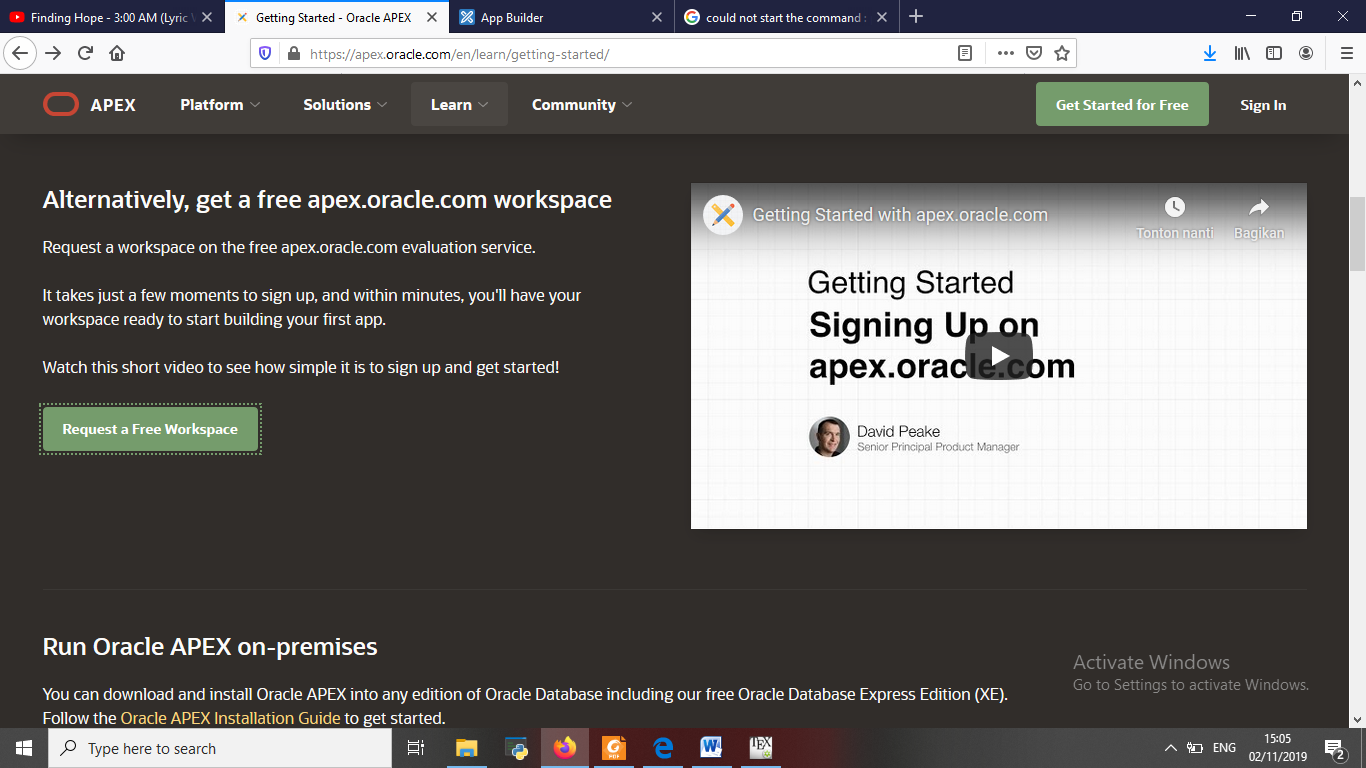
\includegraphics[scale=0.5]{gambar/0.JPG}
    \label{penanda}
\end{figure}

    \item Pada survey, klik yes pada kedua pertanyaan seperti gambar berikut ini.
    \item Setelah survey, isi justification dan klik next
    \item Lalu, pada agreement klik i accept the terms dan klik next.
    \item Selanjutnya confirmation dan submit workspace yang akan dibuat.
    
\begin{figure}[!htbp]
    \centering
    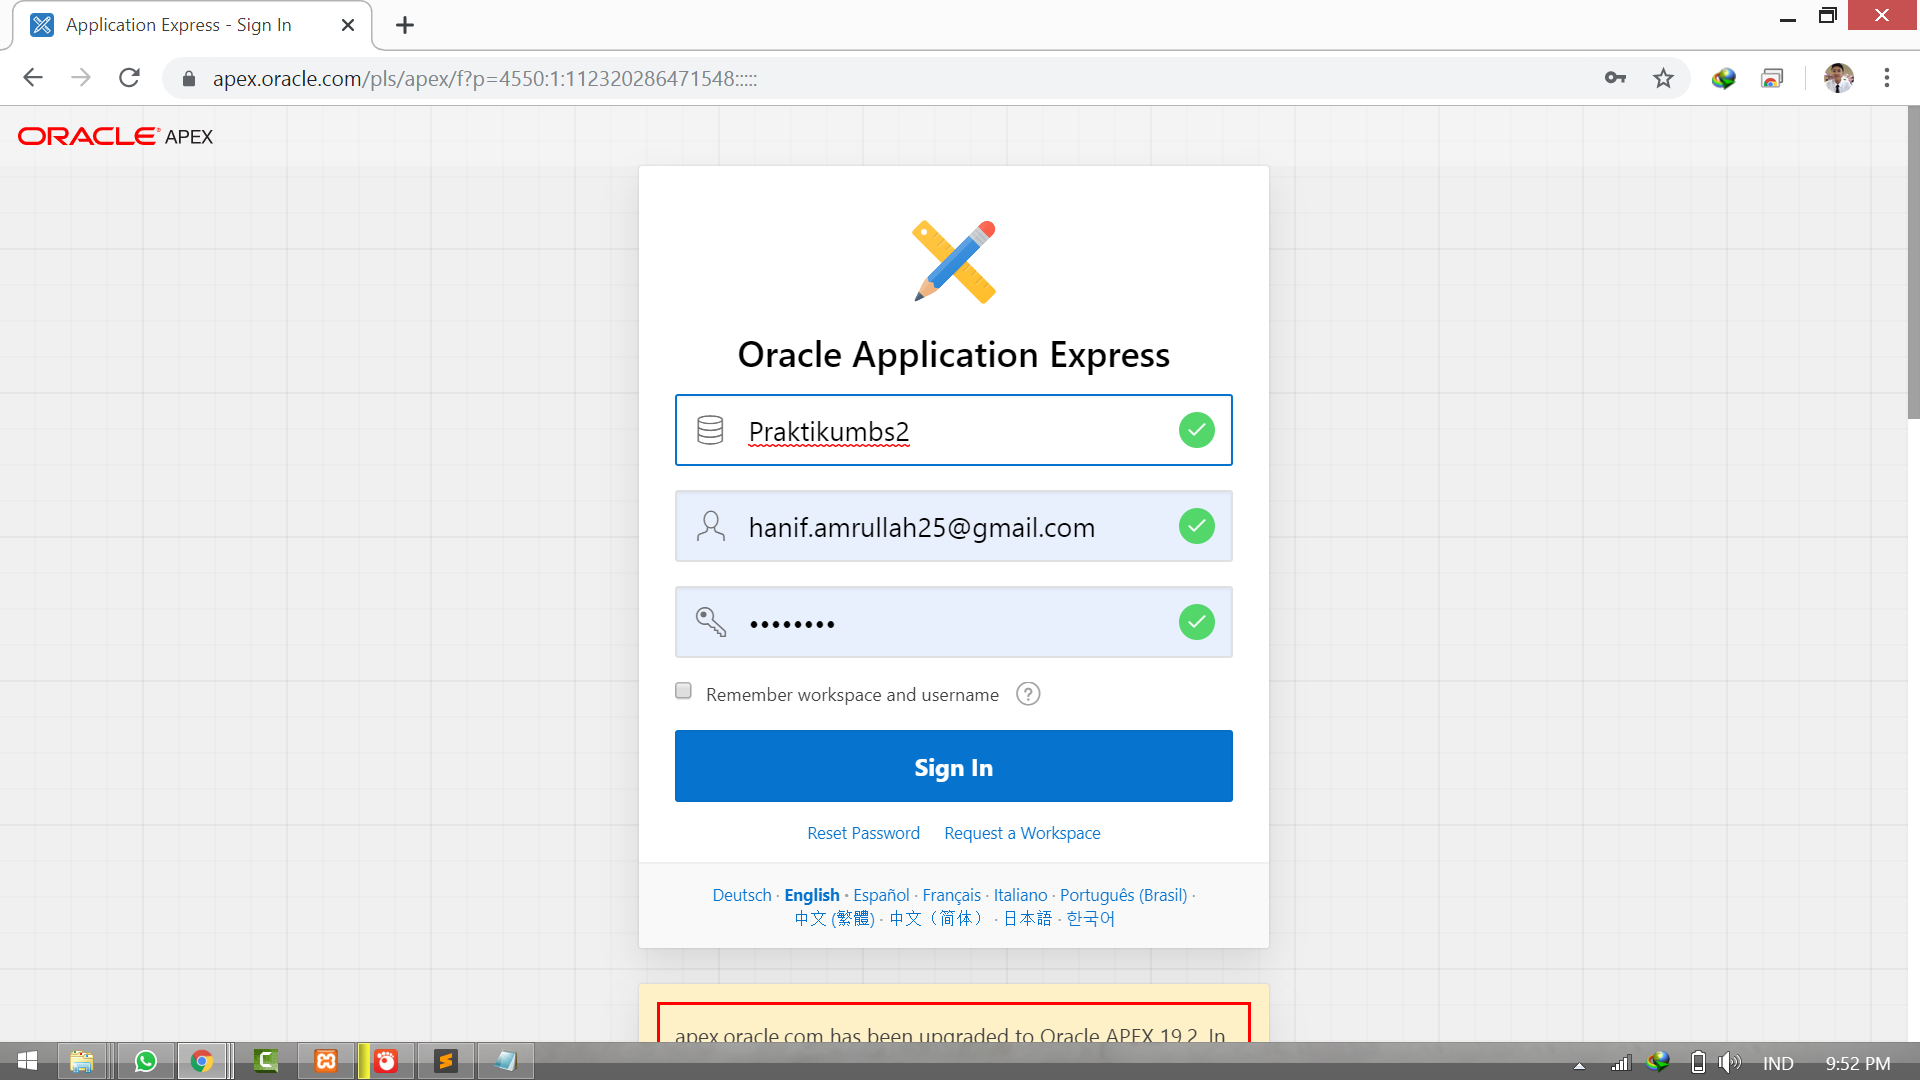
\includegraphics[scale=0.5]{gambar/1.JPG}
    \label{penanda}
\end{figure}
    
\begin{figure}[!htbp]
    \centering
    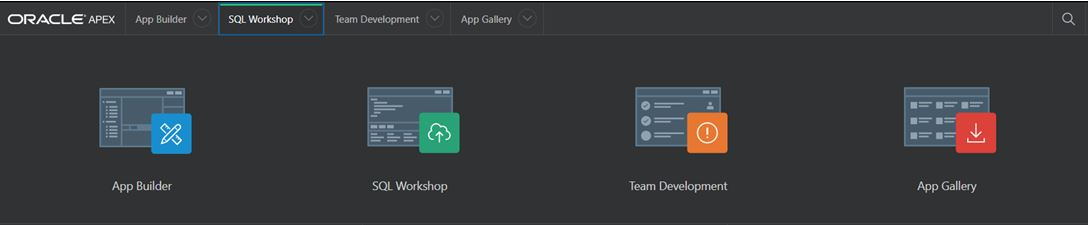
\includegraphics[scale=0.5]{gambar/2.JPG}
    \label{penanda}
\end{figure}

\begin{figure}[!htbp]
    \centering
    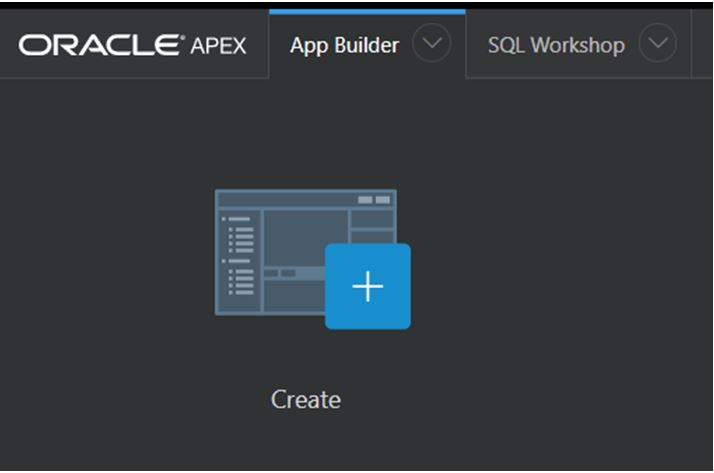
\includegraphics[scale=0.5]{gambar/3.JPG}
    \label{penanda}
\end{figure}

\begin{figure}[!htbp]
    \centering
    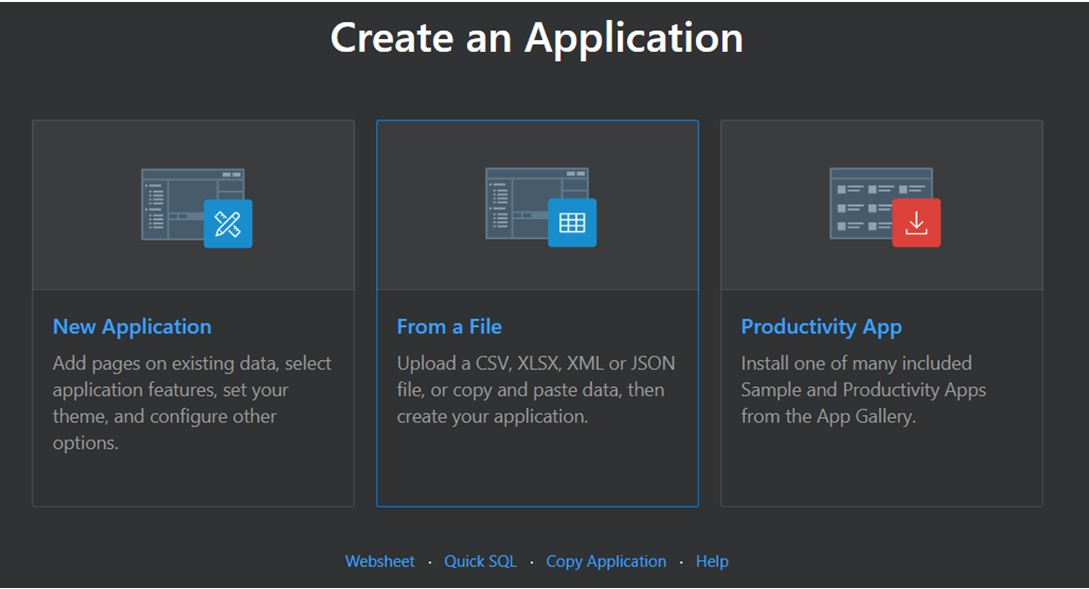
\includegraphics[scale=0.5]{gambar/4.JPG}
    \label{penanda}
\end{figure}

\begin{figure}[!htbp]
    \centering
    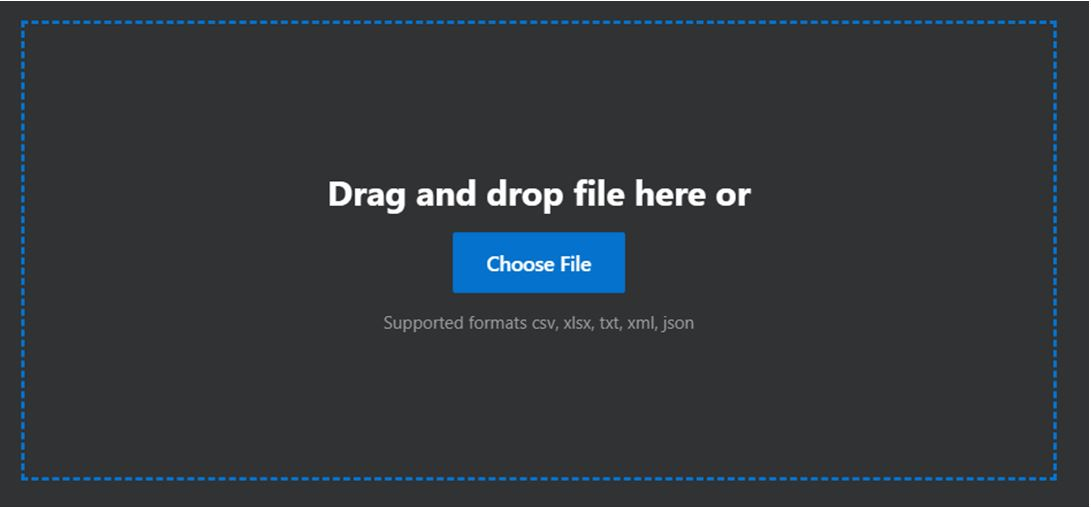
\includegraphics[scale=0.5]{gambar/5.JPG}
    \label{penanda}
\end{figure}
\begin{figure}[!htbp]
    \centering
    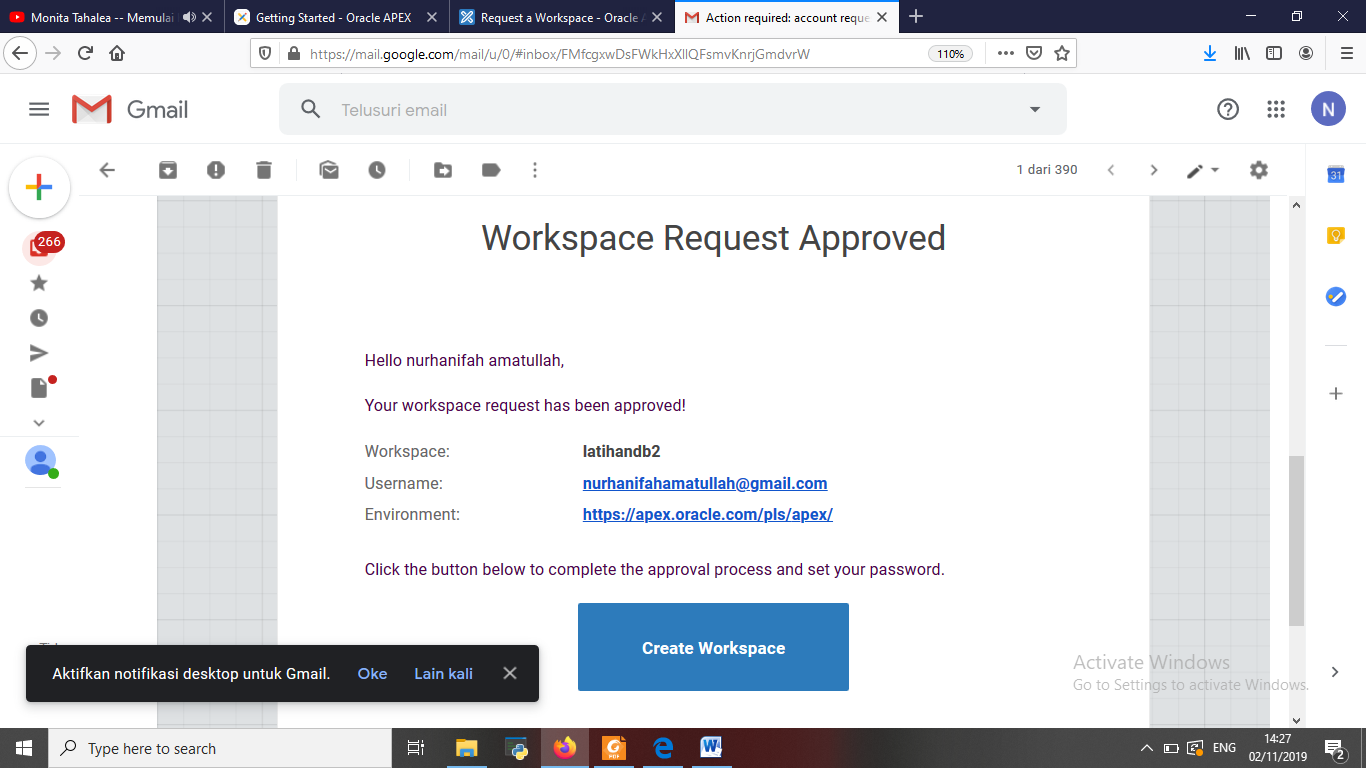
\includegraphics[scale=0.5]{gambar/6.JPG}
    \label{penanda}
\end{figure}

\end{enumerate}

\section{Konfirmasi Email Workspace}

\begin{enumerate}
    \item Buka email dan klik kotak masuk
    \item Klik email dari apex oracle
    \item Berikut ini adalah tampilan email dari apex oracle yang sudah di verifikasi.
    
    \item Setelah workspace berhasil dibuat, masukkan password untuk workspace yang telah dibuat tadi

\begin{figure}[!htbp]
    \centering
    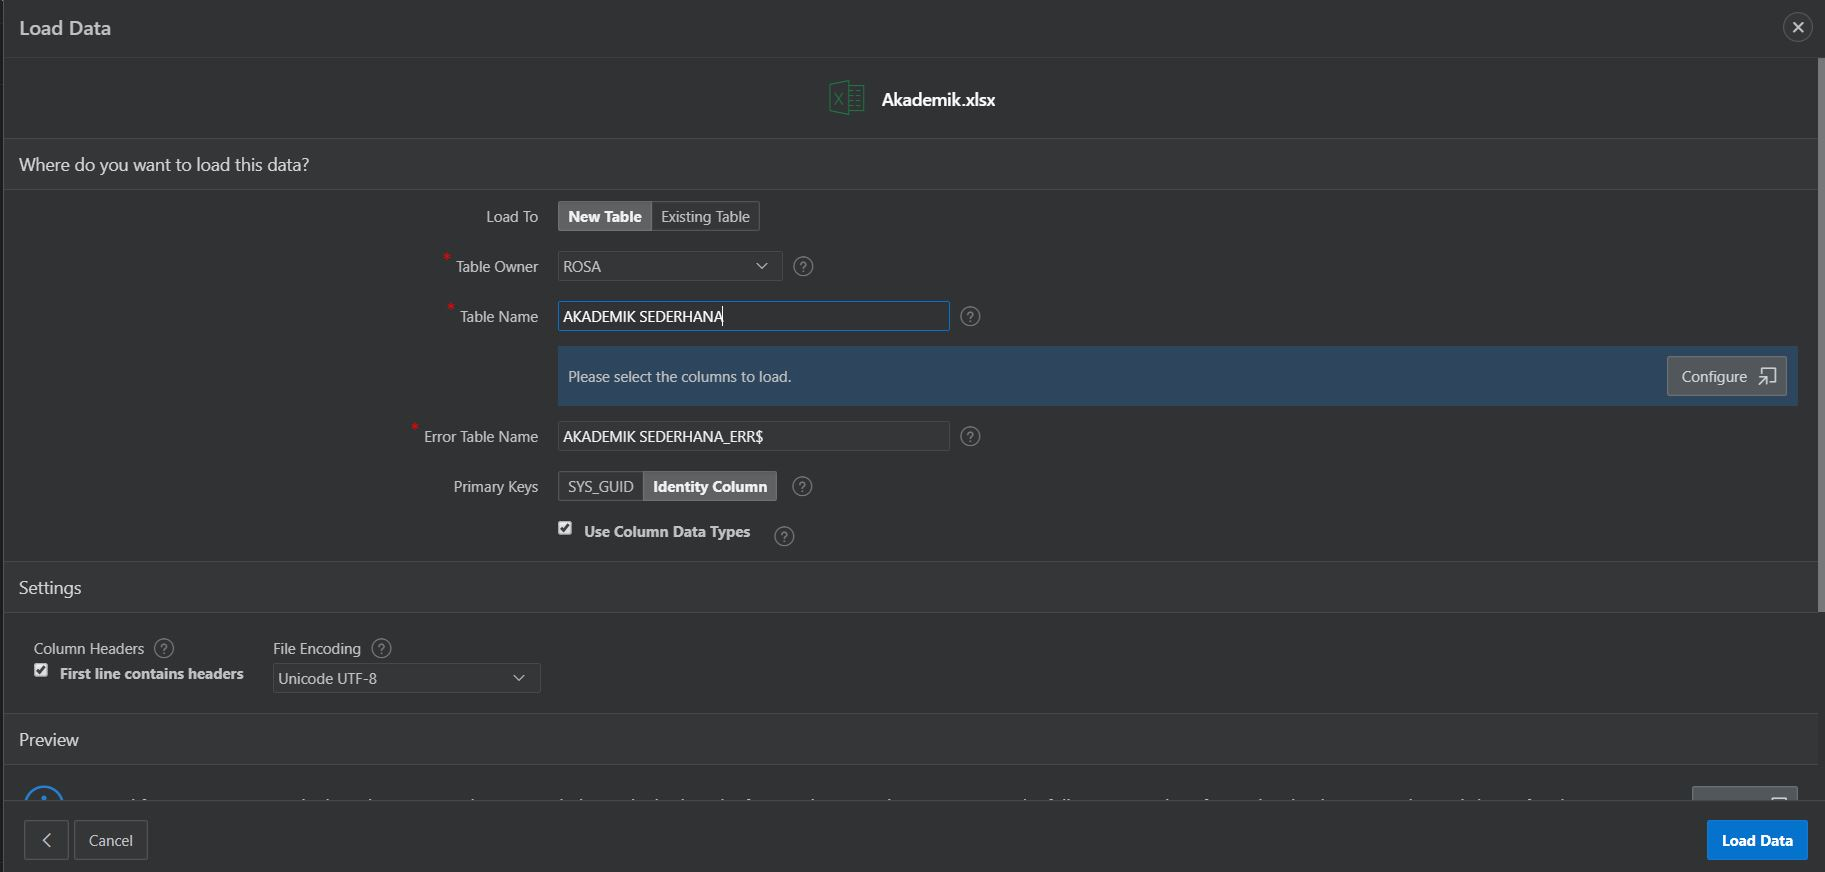
\includegraphics[scale=0.5]{gambar/7.JPG}
    \label{penanda}
\end{figure}

    \item Workspace berhasil dibuat
 
\end{enumerate}
\vspace{6cm}
\section{Membuat Aplikasi Akademik dari Data Excel}.
\begin{enumerate}
    \item Setelah sig in ke workspace APEX Oracle, klik app builder
    \item Pada halaman app builder, klik create untuk membuat aplikasi

\begin{figure}[!htbp]
    \centering
    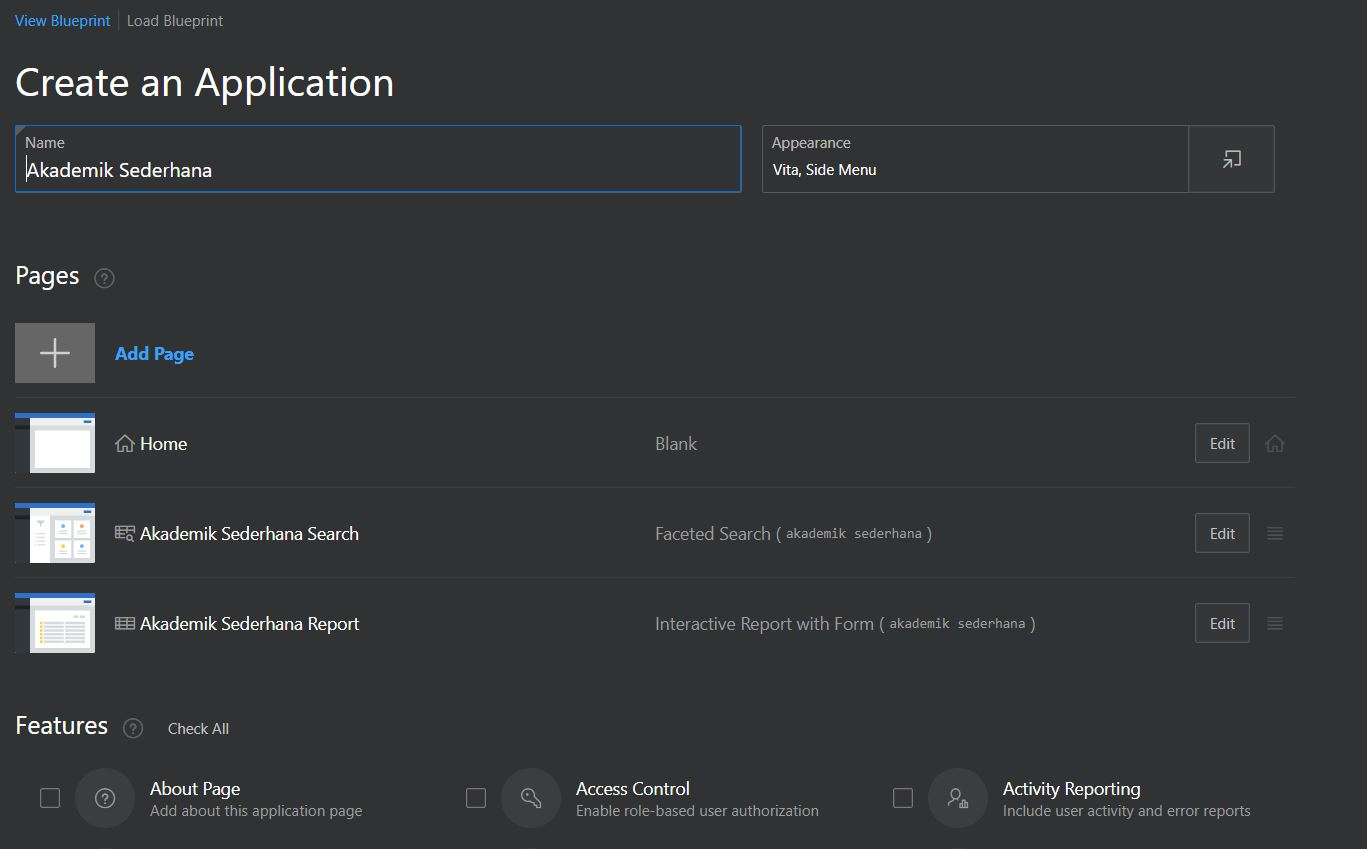
\includegraphics[scale=0.5]{gambar/10.JPG}
    \label{penanda}
\end{figure}

    \item Arahkan kursor ke from a file untuk mengupload data excel
    \item Selanjutnya drop file excel

\begin{figure}[!htbp]
    \centering
    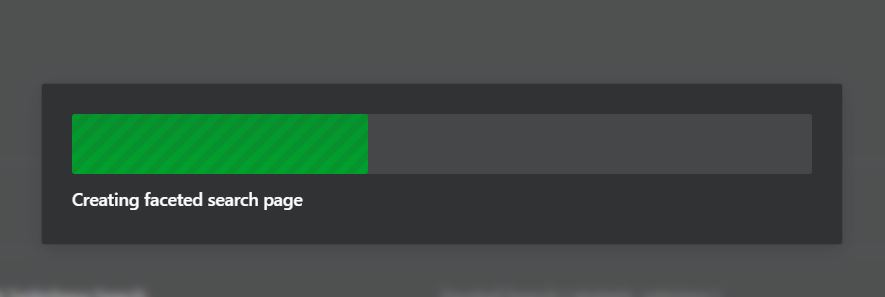
\includegraphics[scale=0.5]{gambar/11.JPG}
    \label{penanda}
\end{figure}

    \item Setelah file di drop, input nama table, dan load data
    \item Setelah table dibuat, klik create application
    \item Input nama aplikasi, aplikasi ini saya namakan aplikasi akademik
    \item Lalu, klik check all dan create application
    
\begin{figure}[!htbp]
    \centering
    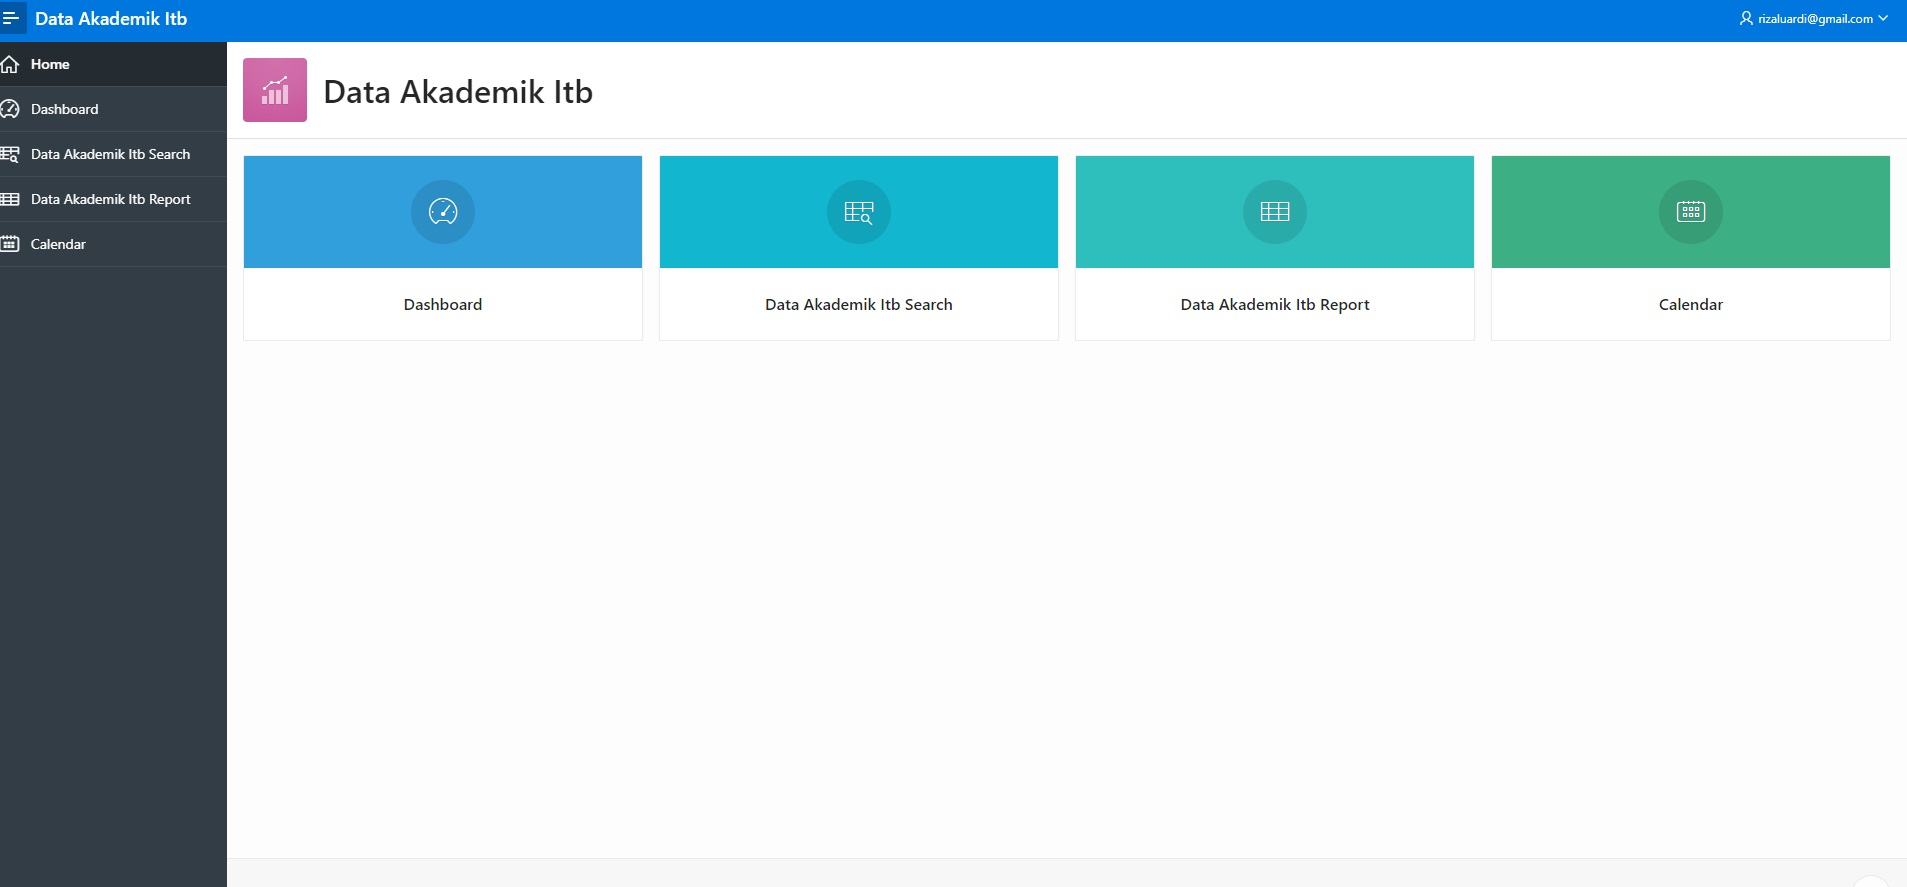
\includegraphics[scale=0.5]{gambar/12.JPG}
    \label{penanda}
\end{figure}

\begin{figure}[!htbp]
    \centering
    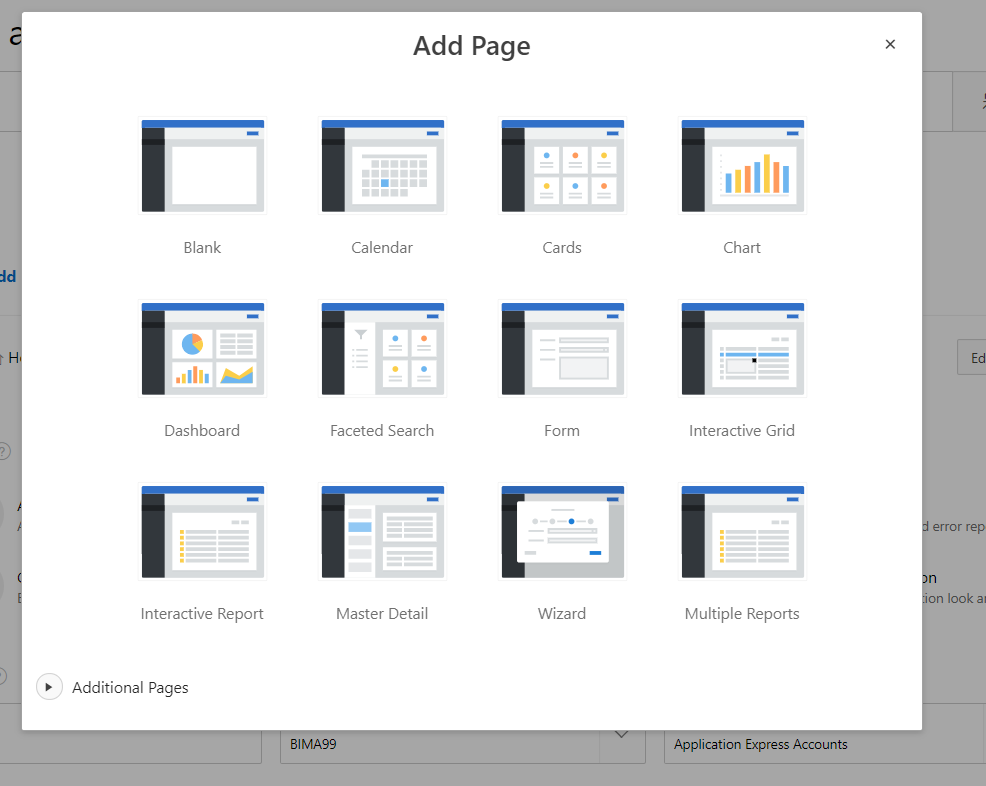
\includegraphics[scale=0.5]{gambar/14.JPG}
    \label{penanda}
\end{figure}
    
    \item Setelah aplikasi terbuat, running aplikasi dengan klik run application
    \item Aplikasi akan berjalan dan mengarah ke halaman baru. Untuk membuka aplikasi, log in terlebih dahulu menggunakan user APEX Oracle dan password pada workspace yang digunakan.

    \item link : https://apex.oracle.com/pls/apex/f?p=78972:3:6747675556863::NO:::
    \item {email: kurniahayati907@gmail.com}
    \item {pass: kurniahayati25}
    
\end{enumerate}